\documentclass{article}
\usepackage{comment}
\usepackage{graphicx} % Required for inserting images
\usepackage[compat=1.0.0]{tikz-feynman} % For Feynman diagram drawings 
\usepackage{xcolor}
\title{VBS diagram: $ZZ \rightarrow 4l$ final state}
\author{}
\date{}

\begin{document}
\maketitle
\newpage

\section*{Generic VBS diagrams}

\begin{center}
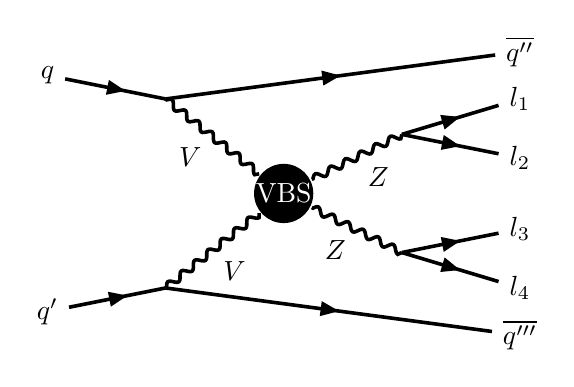
\begin{tikzpicture}[scale=1.5, line width=1.3pt]
\begin{feynman}

\vertex (i1) at (-1,1) {$q$};
\vertex (i2) at (-1,-1) {$q'$};

\vertex (a) at (0,0.8);
\vertex (b) at (0,-0.8);
% Blob
% Interaction blob
\node[
    circle,
    fill=black,
    minimum size=5mm,
    inner sep=0pt
] (v) at (1,0) {\color{white}{VBS}};

\vertex (e) at (2,0.5);
\vertex (f) at (2,-0.5);

\vertex (l1) at (3,0.8) {$l_1$};
\vertex (l2) at (3,0.3) {$l_2$};
\vertex (l3) at (3,-0.3) {$l_3$};
\vertex (l4) at (3,-0.8) {$l_4$};


\vertex (f1) at (3,1.2)  {$\overline{q''}$}; 
\vertex (f2) at (3,-1.2) {$\overline{q'''}$};

\diagram*{
  (i1) -- [fermion] (a),
  (i2) -- [fermion] (b),
  (a) -- [fermion] (f1),
  (b) -- [fermion] (f2),
  
  (a) -- [boson, edge label'=\(V\)] (v),
  (b) -- [boson, edge label'=\(V\)] (v),
   
  
  (v) -- [boson, edge label'=\(Z\)] (e),
  (v) -- [boson, edge label'=\(Z\)] (f),

  (e) -- [fermion] (l1),
  (e) -- [fermion] (l2),
  (f) -- [fermion] (l3),
  (f) -- [fermion] (l4),
};

\end{feynman}
\end{tikzpicture}
\end{center}

\section*{t-Channel W mediated ZZ}

\begin{center}
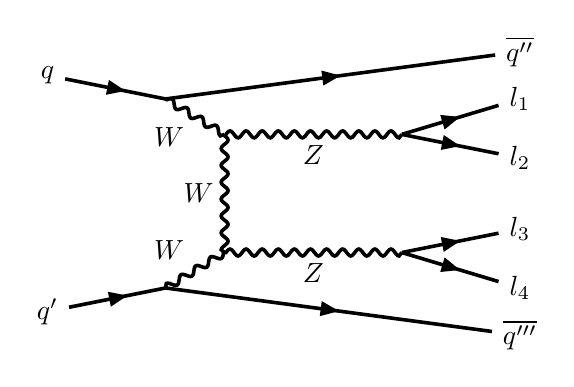
\begin{tikzpicture}[scale=1.5, line width=1.3pt]
\begin{feynman}

\vertex (i1) at (-1,1) {$q$};
\vertex (i2) at (-1,-1) {$q'$};

\vertex (a) at (0,0.8);
\vertex (b) at (0.5,0.5);
\vertex (c) at (0.5,-0.5); 
\vertex (d) at (0,-0.8);
\vertex (e) at (2,0.5);
\vertex (f) at (2,-0.5);

\vertex (l1) at (3,0.8) {$l_1$};
\vertex (l2) at (3,0.3) {$l_2$};
\vertex (l3) at (3,-0.3) {$l_3$};
\vertex (l4) at (3,-0.8) {$l_4$};


\vertex (f1) at (3,1.2)  {$\overline{q''}$}; 
\vertex (f2) at (3,-1.2) {$\overline{q'''}$};

\diagram*{
  (i1) -- [fermion] (a),
  (i2) -- [fermion] (d),
  (a) -- [fermion] (f1),
  (d) -- [fermion] (f2),
  
  (a) -- [boson, edge label'=\(W\)] (b),
  (b) -- [boson, edge label'=\(W\)] (c),
  (c) -- [boson, edge label'=\(W\)] (d),
  
  (b) -- [boson, edge label'=\(Z\)] (e),
  (c) -- [boson, edge label'=\(Z\)] (f),

  (e) -- [fermion] (l1),
  (e) -- [fermion] (l2),
  (f) -- [fermion] (l3),
  (f) -- [fermion] (l4),
};

\end{feynman}
\end{tikzpicture}
\end{center}

\section*{s-channel Higgs ZZ}

\begin{center}
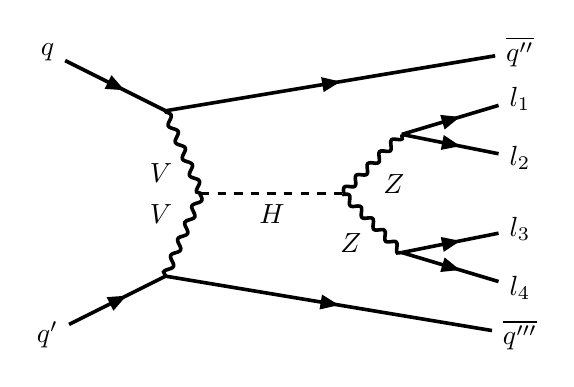
\begin{tikzpicture}[scale=1.5, line width = 1.3pt]
\begin{feynman}

\vertex (i1) at (-1,1.2) {$q$};
\vertex (i2) at (-1,-1.2) {$q'$};

\vertex (a) at (0,0.7);
\vertex (b) at (0.3,0);
\vertex (c) at (0,-0.7);

\vertex (d) at (1.5,0);
\vertex (e) at (2,0.5);
\vertex (f) at (2,-0.5);

\vertex (l1) at (3,0.8) {$l_1$};
\vertex (l2) at (3,0.3) {$l_2$};
\vertex (l3) at (3,-0.3) {$l_3$};
\vertex (l4) at (3,-0.8) {$l_4$};

\vertex (f1) at (3,1.2)  {$\overline{q''}$}; 
\vertex (f2) at (3,-1.2) {$\overline{q'''}$};

\diagram*{
  (i1) -- [fermion] (a),
  (i2) -- [fermion] (c),
  (a) -- [fermion] (f1),
  (c) -- [fermion] (f2),
  
  (a) -- [boson, edge label'=\(V\)] (b),
  (b) -- [boson, edge label'=\(V\)] (c),

  (b) -- [scalar, edge label'=\(H\)] (d),
  
  (d) -- [boson, edge label'=\(Z\)] (e),
  (d) -- [boson, edge label'=\(Z\)] (f),

  (e) -- [fermion] (l1),
  (e) -- [fermion] (l2),
  (f) -- [fermion] (l3),
  (f) -- [fermion] (l4),
};

\end{feynman}
\end{tikzpicture}
\end{center}

\section*{t-Channel Higgs ZZ}
\begin{center}
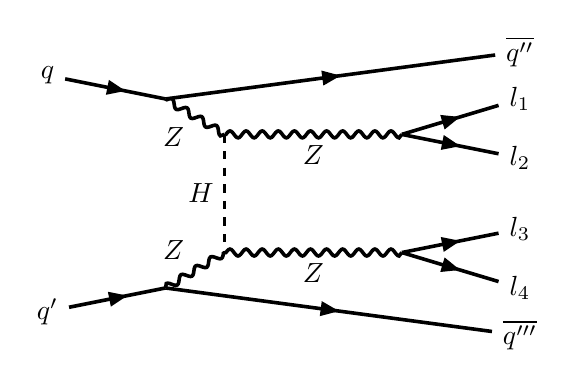
\begin{tikzpicture}[scale=1.5, line width=1.3pt]
\begin{feynman}

\vertex (i1) at (-1,1) {$q$};
\vertex (i2) at (-1,-1) {$q'$};

\vertex (a) at (0,0.8);
\vertex (b) at (0.5,0.5);
\vertex (c) at (0.5,-0.5); 
\vertex (d) at (0,-0.8);
\vertex (e) at (2,0.5);
\vertex (f) at (2,-0.5);

\vertex (l1) at (3,0.8) {$l_1$};
\vertex (l2) at (3,0.3) {$l_2$};
\vertex (l3) at (3,-0.3) {$l_3$};
\vertex (l4) at (3,-0.8) {$l_4$};


\vertex (f1) at (3,1.2)  {$\overline{q''}$}; 
\vertex (f2) at (3,-1.2) {$\overline{q'''}$};

\diagram*{
  (i1) -- [fermion] (a),
  (i2) -- [fermion] (d),
  (a) -- [fermion] (f1),
  (d) -- [fermion] (f2),
  
  (a) -- [boson, edge label'=\(Z\)] (b),
  (b) -- [scalar, edge label'=\(H\)] (c),
  (c) -- [boson, edge label'=\(Z\)] (d),
  
  (b) -- [boson, edge label'=\(Z\)] (e),
  (c) -- [boson, edge label'=\(Z\)] (f),

  (e) -- [fermion] (l1),
  (e) -- [fermion] (l2),
  (f) -- [fermion] (l3),
  (f) -- [fermion] (l4),
};

\end{feynman}
\end{tikzpicture}
\end{center}

\section*{Quartic Coupling}

\begin{center}
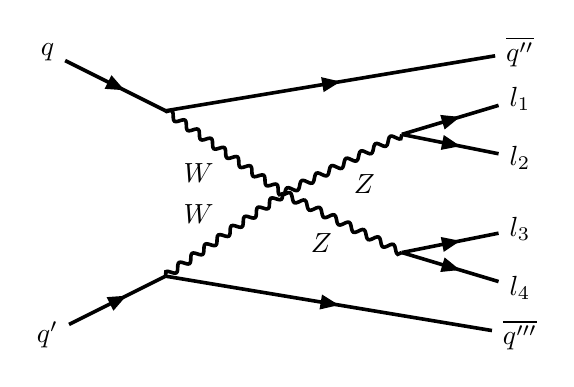
\begin{tikzpicture}[scale=1.5, line width = 1.3pt]
\begin{feynman}

\vertex (i1) at (-1,1.2) {$q$};
\vertex (i2) at (-1,-1.2) {$q'$};

\vertex (a) at (0,0.7);
\vertex (b) at (1,0);
\vertex (c) at (0,-0.7);
\vertex (e) at (2,0.5);
\vertex (f) at (2,-0.5);

\vertex (l1) at (3,0.8) {$l_1$};
\vertex (l2) at (3,0.3) {$l_2$};
\vertex (l3) at (3,-0.3) {$l_3$};
\vertex (l4) at (3,-0.8) {$l_4$};

\vertex (f1) at (3,1.2)  {$\overline{q''}$}; 
\vertex (f2) at (3,-1.2) {$\overline{q'''}$};

\diagram*{
  (i1) -- [fermion] (a),
  (i2) -- [fermion] (c),
  (a) -- [fermion] (f1),
  (c) -- [fermion] (f2),
  
  (a) -- [boson, edge label'=\(W\)] (b),
  (b) -- [boson, edge label'=\(W\)] (c),  
  (b) -- [boson, edge label'=\(Z\)] (e),
  (b) -- [boson, edge label'=\(Z\)] (f),

  (e) -- [fermion] (l1),
  (e) -- [fermion] (l2),
  (f) -- [fermion] (l3),
  (f) -- [fermion] (l4),
};

\end{feynman}
\end{tikzpicture}
\end{center}

\section*{Generic VBS diagrams}

\begin{center}
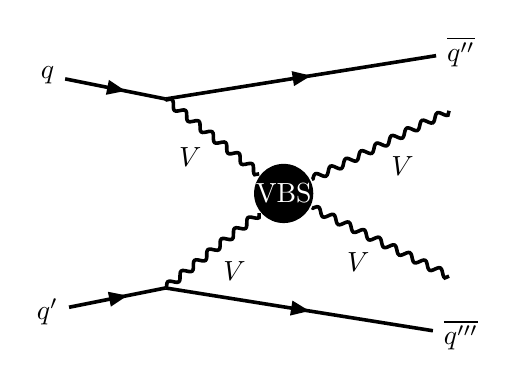
\begin{tikzpicture}[scale=1.5, line width=1.3pt]
\begin{feynman}

\vertex (i1) at (-1,1) {$q$};
\vertex (i2) at (-1,-1) {$q'$};

\vertex (a) at (0,0.8);
\vertex (b) at (0,-0.8);
% Blob
% Interaction blob
\node[
    circle,
    fill=black,
    minimum size=5mm,
    inner sep=0pt
] (v) at (1,0) {\color{white}{VBS}};

\vertex (e) at (2.4,0.7);
\vertex (f) at (2.4,-0.7);

\vertex (f1) at (2.5,1.2)  {$\overline{q''}$}; 
\vertex (f2) at (2.5,-1.2) {$\overline{q'''}$};

\diagram*{
  (i1) -- [fermion] (a),
  (i2) -- [fermion] (b),
  (a) -- [fermion] (f1),
  (b) -- [fermion] (f2),
  
  (a) -- [boson, edge label'=\(V\)] (v),
  (b) -- [boson, edge label'=\(V\)] (v),
   
  
  (v) -- [boson, edge label'=\(V\)] (e),
  (v) -- [boson, edge label'=\(V\)] (f),

};
\end{feynman}
\end{tikzpicture}
\end{center}

\section*{Polarized modes of Vector bosons}
\begin{center}
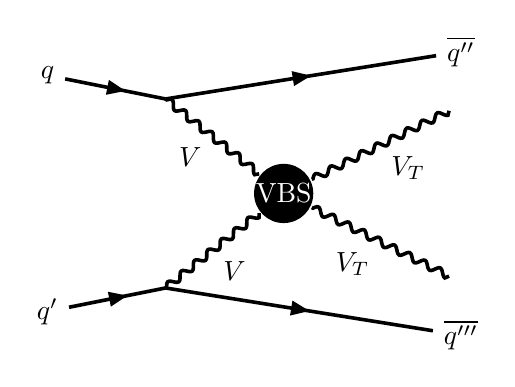
\begin{tikzpicture}[scale=1.5, line width=1.3pt]
\begin{feynman}

\vertex (i1) at (-1,1) {$q$};
\vertex (i2) at (-1,-1) {$q'$};

\vertex (a) at (0,0.8);
\vertex (b) at (0,-0.8);
% Blob
% Interaction blob
\node[
    circle,
    fill=black,
    minimum size=5mm,
    inner sep=0pt
] (v) at (1,0) {\color{white}{VBS}};

\vertex (e) at (2.4,0.7);
\vertex (f) at (2.4,-0.7);

\vertex (f1) at (2.5,1.2)  {$\overline{q''}$}; 
\vertex (f2) at (2.5,-1.2) {$\overline{q'''}$};

\diagram*{
  (i1) -- [fermion] (a),
  (i2) -- [fermion] (b),
  (a) -- [fermion] (f1),
  (b) -- [fermion] (f2),
  
  (a) -- [boson, edge label'=\(V\)] (v),
  (b) -- [boson, edge label'=\(V\)] (v),
   
  
  (v) -- [boson, edge label'=\(V_T\)] (e),
  (v) -- [boson, edge label'=\(V_T\)] (f),

};
\end{feynman}
\end{tikzpicture}
\end{center}


\end{document}
